\section{CTL Commands}

\subsection{ctl}
Das Hauptkommando. Hierüber besteht Zugriff auf alle anderen Befehle wie
\lstlisting{git} es tun würde.

So kann z.B. das Kommando \lstlisting[language=Bash]{ctl register test.com} die
Domain \emph{test.com} als Webinstance hinzufügen.
Für nähere Informationen ist
die Dokumentation oder Manualpage zu konsultieren.


\subsection{ctl-genmanifest}

Dieser Befehl generiert eine Manifest-Datei aus einer CTL Compontent. Er ist zur
Verwendung von Component Entwicklern gedacht.


\subsection{ctl-web}

\lstlisting[language=Bash]{ctl-web} stellt die Schnittstelle für ein
Webinterface zum Backend bereit. Mit dem Kommando können neue Benutzer für den
CTL-Zugriff registriert werden.

Umgesetzt wird das indem der/die public SSH Schlüssel in die
\emph{.ssh/authorized_keys} eingetragen werden.

Parameter:
--add 


\subsection{ctl-init}

\lstlisting[language=Bash]{ctl-init} steht für die Benutzer einer Component
bereit um eine solche zu spawnen. Benutzer die mit
\lstlisting[language=Bash]{ctl-web} hinzugefügt wurden bekommen nur auf diese
Kommando zugriff und können keine weiteren Befehle starten.


\subsection{ctl-runcgi}




\subsection{ctl-register}

\section{Entwürfe}

\subsection[Datenbank}
\begin{figure}[h]
\centering
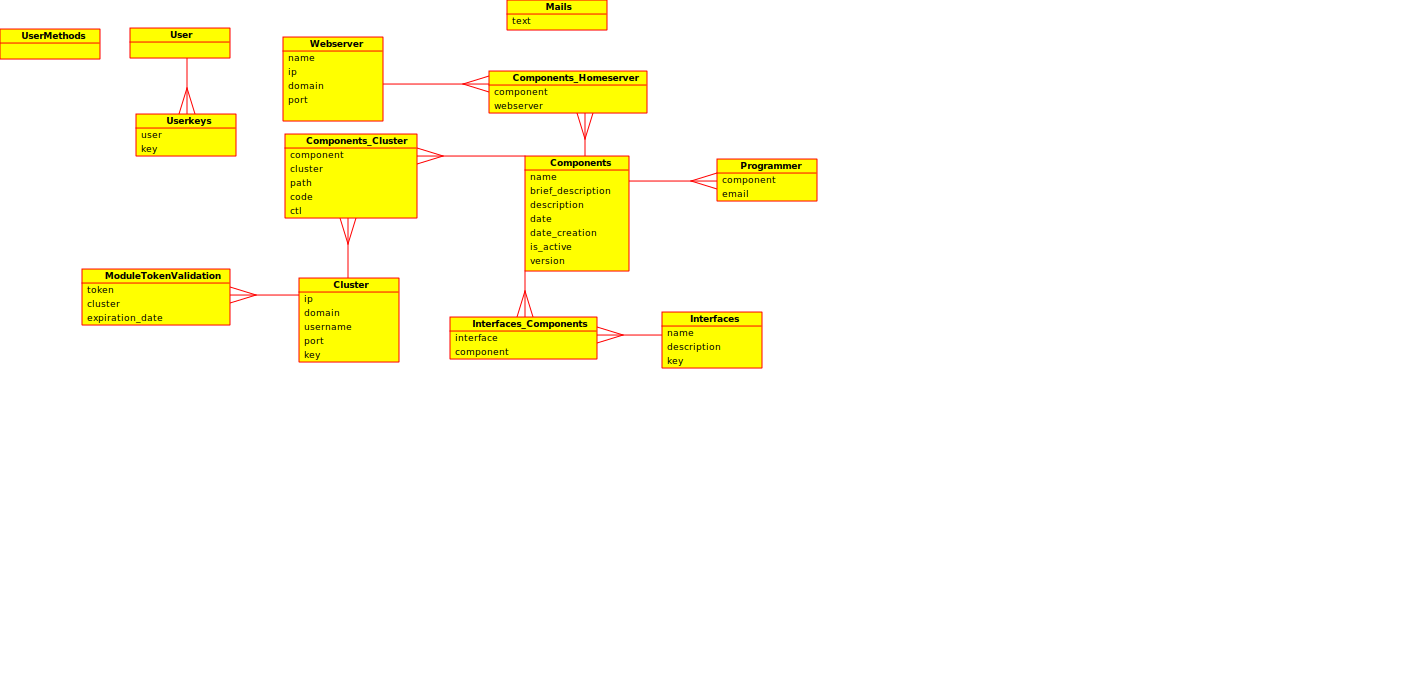
\includegraphics[width=0.8\linewidth]{Bilder/ctl-db.svg}
\caption[CTL-DB]{CTL-DB}
\label{CTL-Datenbank}
\end{figure}
